% Plate diagram of the angle likelihood (manual §2.5), rendered by docs/make_plate_diagram.jl.
% Hyperparameters are named as the fields of PhyllotaxisPrior and TorsionPrior.
\documentclass[tikz, border = 2pt]{standalone}
\usetikzlibrary{bayesnet, backgrounds, arrows.meta}

\tikzset{
  >= {Stealth[length = 5pt, width = 4pt]},
  every edge/.append style = {draw = black!75, line width = 0.5pt},
  latent/.append style = {minimum size = 30pt, line width = 0.6pt},
  obs/.append style = {minimum size = 30pt, line width = 0.6pt},
  hyper/.style = {rectangle, draw = black!40, dashed, text = black!65, font = \small, inner sep = 3pt,
    minimum height = 15pt, rounded corners = 1pt},
  covariate/.style = {rectangle, draw, fill = gray!25, minimum size = 24pt, inner sep = 1pt, line width = 0.6pt},
  summed/.style = {latent, double, double distance = 1.2pt},
  plate caption/.append style = {font = \small},
}

\begin{document}
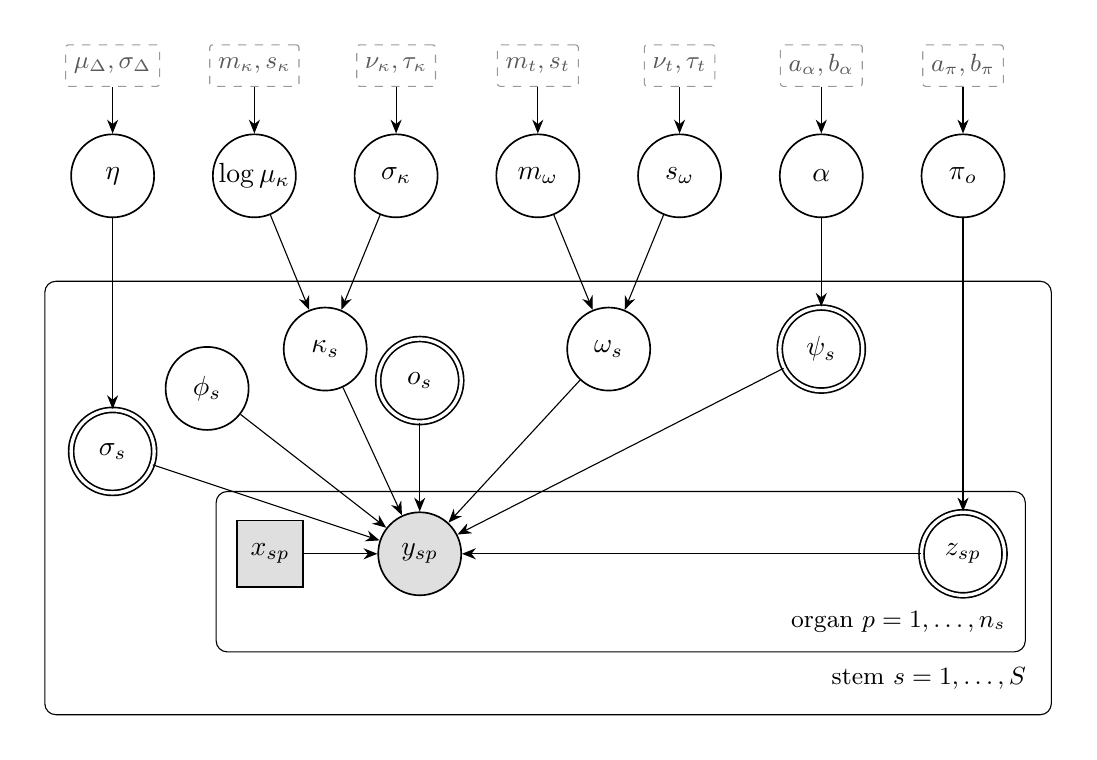
\begin{tikzpicture}[show background rectangle,
    background rectangle/.style = {fill = white}, inner frame sep = 6pt]

  % hyperparameters
  \node[hyper] (heta) at (0.3, 0)    {$\mu_\Delta, \sigma_\Delta$};
  \node[hyper] (hmu)  at (2.1, 0)  {$m_\kappa, s_\kappa$};
  \node[hyper] (hsig) at (3.9, 0)  {$\nu_\kappa, \tau_\kappa$};
  \node[hyper] (hm)   at (5.7, 0)  {$m_t, s_t$};
  \node[hyper] (hs)   at (7.5, 0)  {$\nu_t, \tau_t$};
  \node[hyper] (halp) at (9.3, 0)  {$a_\alpha, b_\alpha$};
  \node[hyper] (hpi)  at (11.1, 0) {$a_\pi, b_\pi$};

  % population parameters
  \node[latent] (eta)    at (0.3, -1.4)    {$\eta$};
  \node[latent] (mukap)  at (2.1, -1.4)  {$\log\mu_\kappa$};
  \node[latent] (sigkap) at (3.9, -1.4)  {$\sigma_\kappa$};
  \node[latent] (mom)    at (5.7, -1.4)  {$m_\omega$};
  \node[latent] (som)    at (7.5, -1.4)  {$s_\omega$};
  \node[latent] (alp)    at (9.3, -1.4)  {$\alpha$};
  \node[latent] (pio)    at (11.1, -1.4) {$\pi_o$};

  % stem: the parents of y on an arc above it
  \node[summed] (ord) at (0.3, -4.9)   {$\sigma_s$};
  \node[latent] (phi) at (1.5, -4.1) {$\phi_s$};
  \node[latent] (kap) at (3.0, -3.6) {$\kappa_s$};
  \node[summed] (o)   at (4.2, -4.0) {$o_s$};
  \node[latent] (om)  at (6.6, -3.6) {$\omega_s$};
  \node[summed] (psi) at (9.3, -3.6) {$\psi_s$};

  % organ
  \node[obs]       (y) at (4.2, -6.2)  {$y_{sp}$};
  \node[covariate] (x) at (2.3, -6.2)  {$x_{sp}$};
  \node[summed]    (z) at (11.1, -6.2) {$z_{sp}$};

  \edge {heta} {eta}; \edge {hmu} {mukap}; \edge {hsig} {sigkap}; \edge {hm} {mom}; \edge {hs} {som};
  \edge {halp} {alp}; \edge {hpi} {pio};
  \edge {eta} {ord}; \edge {mukap, sigkap} {kap}; \edge {mom, som} {om}; \edge {alp} {psi}; \edge {pio} {z};
  \edge {ord, phi, kap, o, om, psi, x, z} {y};

  \plate[inner sep = 7pt] {organ} {(y) (x) (z)} {organ $p = 1, \dots, n_s$};
  \plate[inner sep = 9pt] {stem} {(ord) (phi) (kap) (o) (om) (psi) (organ)} {stem $s = 1, \dots, S$};
\end{tikzpicture}
\end{document}
